\documentclass[12pt]{article}
\usepackage{amsmath, amssymb}
\usepackage{graphicx}
\usepackage{float}
\usepackage[letterpaper, margin=1in]{geometry}

\begin{document}
\pagestyle{empty}

\begin{center}
    \Huge \textbf{Introduction}
\end{center}

Shohei Ohtani is an MLB player for the Los Angeles Dodgers and formerly for the Los Angeles Angels. He is unique in that he both bats and pitches, something rare in professional baseball. Even more rare, he is elite at both. In 2022, he finished 4th in Cy Young voting (the best pitcher award) and 2nd in MVP voting (the best player award). He is a 4x MVP winner, having won in 2021 and 2023-2025. He has won the Silver Slugger Award (best hitter at his position) 4x. He also won rookie of the year. He has revolutionized baseball by being such a so-called unicorn; he is truly a once-in-a-generation type of player.

The question I am attempting to answer is whether Shohei hits differently when he’s pitching than when he's only batting. I chose this topic because I’m a sports and baseball fan. I’m interested in what makes a player great, and what factors can affect a great player, which naturally led me to this question. Going into this project, I think that there will not be a difference because the effects of pitching fatigue will balance out with being more focused and engaged with the game, something that MLB players say has a huge impact on their performance (see Rafael Dever’s breakup with the Red Sox over not being able to play in the field, an effect I’d imagine would only be increased by pitching due to the even more greater focus needed).

To analyze Shohei’s performance on a game-by-game basis, I'll use a stat called wOBA (weighted on-base average). wOBA is defined by the equation
\[\text{wOBA} = \frac{
        0.69 \cdot \text{NIBB} +
        0.722 \cdot \text{HBP} +
        0.881 \cdot \text{1B} +
        1.257 \cdot \text{2B} +
        1.593 \cdot \text{3B} +
        2.058 \cdot \text{HR}
    }{
        \text{AB} + \text{BB} - \text{IBB} + \text{SF} + \text{HBP}
    }.
\]

If you’re not familiar with wOBA, it’s not overly important. You can study the chart below, which shows a good rule of thumb for assessing wOBA.
\begin{figure}[H]
    \centering
    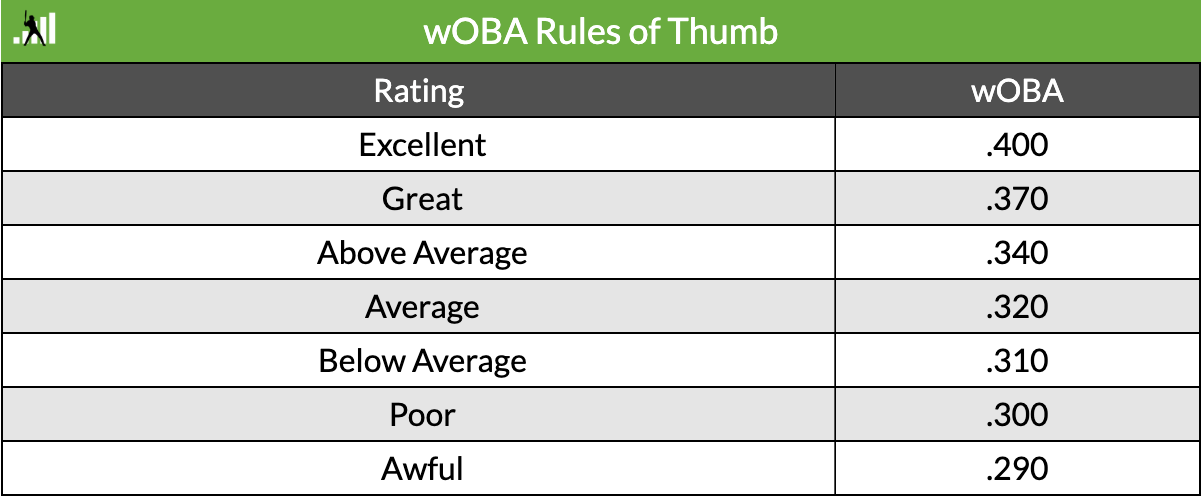
\includegraphics[width=1\textwidth]{woba_chart.png}
\end{figure}

The data I am using is every regular-season game Shohei played from 2021 to 2023 in which he had at least 3 plate appearances. I chose these years because it was the start of his prime and before he injured his arm, which prevented him from pitching in the entire 2024 season and much of the 2025 season. I treat each game as an observation from a bigger, theoretical population of possible games that describe his true offensive ability during this period. Essentially, the population is the outcomes that would occur had Shohei played an unlimited number of games in this time period. Thus, the games from 2021 to 2023 are a sample from this population, meaning we can infer his true offensive ability with a large sample size.

To analyze the data, I'll generate the wOBA on a per-game basis, then define \(\bar{x}_p\) as the mean wOBA of games in which Shohei pitched, and \(\bar{x}_{np}\) as the mean wOBA of games in which Shohei did not pitch. Then, I’ll perform a 2-sample t-test and a 95\% t-interval for the difference of population means to infer underlying ability. I am using a t-test and t-interval because I am working with means and the population standard deviation is unknown. My parameters of interest are
\begin{align*}
    \mu_p    & = \text{true mean game wOBA when pitching}      \\
    \mu_{np} & = \text{true mean game wOBA when not pitching}.
\end{align*}

My hypotheses are
\begin{align*}
    H_0 & : \mu_p = \mu_{np}     \\
    H_a & : \mu_p \neq \mu_{np}.
\end{align*}
\end{document}